\chapter{Air Quality in Focus: A Smart City Perspective}
\label{chap:OpenDatainSmartCities}

\section{Introduction to Smart Cities}
\label{sec:IntroductionSmartCities}

\subsection{What is a Smart City}

In context of rapid urban population growth, a smart city (SC) is a urban area that uses technology and data-driven solutions to enhance performance, well-being, and reduce costs and resource consumption. The goal of a smart city is to improve the quality of life for its residents by leveraging technology and data to optimize various aspects of urban living, such as transportation, energy efficiency, waste management, public safety, and more. 
Without a universally acknowledged definition for a smart city, an exploration of three distinct definitions is undertaken to foster a comprehensive understanding of the concept and its main pillars.
\\

\textbf{Definition 1}: A smart city is a place where traditional networks and services are made more efficient with the use of digital solutions for the benefit of its inhabitants and business. A smart city goes beyond the use of digital technologies for better resource use and fewer emissions. It means smarter urban transport networks, upgraded water supply and waste disposal facilities, and more efficient ways to light and heat buildings. It also means a more interactive and responsive city administration, safer public spaces, and meeting the needs of an ageing population \cite{foo1}.
\\

\textbf{Definition 2}: A fair and equitable town centered on the citizen that continuously improves its sustainability and resilience, especially the ICTs, to improve the quality of life, the efficiency of urban services innovation, competitiveness without compromising future needs in economic, social, environmental and governance aspects.
\\

\textbf{Definition 3}: The smart city is generally understood as an urban environment characterized by the use of Big Data, digital flows, and networked technologies (Kitchin 2014; Townsend 2013), as well as by experimental approaches to the use of these technologies (Luque-Ayala and Marvin 2015; Tironi and Valderrama 2018), in terms of both governance (Cowley et al 2018; Cowley and Caprotti 2018) and urban and city-regional economic development (Caragliu et al. 2011).
\\

From these three definitions, we can chart six distinct key areas driving the evolution of a smart city \cite{foo2}:

\begin{figure}
\centering
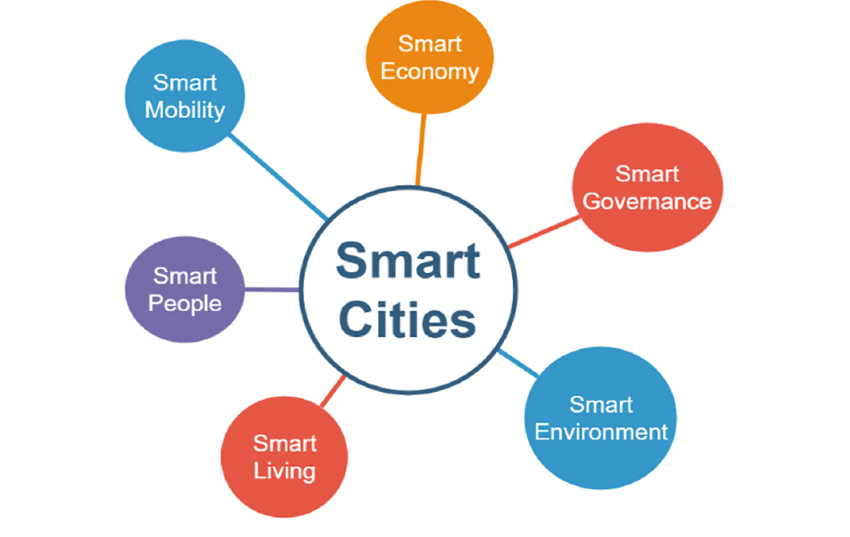
\includegraphics[width=0.7\columnwidth]{images/The-six-pillars-of-Smart-Cities-based-on-8.png}
\caption{The six pillars of Smart Cities \cite{foo3}}
\end{figure}


% Cambiare la forma per evitare l'accapo dell'elenco puntato - FATTO
    

    
 
In a \textbf{Smart Economy}, the focus is on fostering creativity and encouraging entrepreneurial endeavors. This entails cultivating a culture that values \textbf{innovation} and actively supports the initiation of new businesses. The objective is to establish a distinct economic identity through a proactive approach to building trademarks, attracting investments, and gaining global recognition.
Emphasis is placed on optimizing productivity through advanced technologies and adaptable work structures. The labor market's \textbf{flexibility} becomes crucial for resilience in the face of changing economic landscapes. Moreover, active engagement on the international stage is a priority, with a commitment to open trade, collaboration, and continuous transformation for sustained economic growth.

 
The spotlight in a so-defined \textbf{Smart Governance} is on \textbf{citizen participation} in decision-making processes. This involves ensuring that the public is not merely the recipient of policies but an active contributor to shaping them. \textbf{Services} provided by the government, both public and social, are streamlined for efficiency, with a transparent governance structure ensuring accountability and trust.
The long-term vision in political strategies becomes paramount, focusing on sustainability and the well-being of future generations. Smart Governance is characterized by its \textbf{forward-thinking approach}, responsive nature, and a commitment to serving the collective interest of the citizens.


  In a society embracing the principles of \textbf{Smart People}, the primary focus is on education and continuous skill development. The population's high level of qualification becomes the bedrock of innovation and productivity. Lifelong learning is not just encouraged but ingrained as a cultural norm, ensuring \textbf{adaptability to technological advancements}. Diversity, both social and ethnic, is actively celebrated, fostering an environment that values flexibility and creativity. A Smart People society places a premium on a global perspective, encouraging cosmopolitanism and open-mindedness. \textbf{Active participation} in public life is promoted to enhance civic engagement.

    
  \textbf{Smart Mobility} centers around the integration of efficient and interconnected transportation systems. Local accessibility is prioritized through well-connected public transportation, reducing reliance on individual vehicles and contributing to sustainable urban living. International accessibility is also emphasized to enhance cultural exchange and economic activities.
The availability of advanced Information and Communication Technology (ICT) infrastructure is foundational for Smart Mobility. \textbf{Real-time information} empowers individuals to make \textbf{informed transportation choices}, contributing to the reliability and efficiency of transportation networks. \textbf{Sustainability} is a key principle, with a focus on innovative, safe, and eco-friendly transport systems.

 
In a \textbf{Smart environment} the goal is to balance the appeal of natural conditions with responsible environmental practices. \textbf{Pollution control measures} are prioritized, encompassing stringent regulations and sustainable practices to safeguard air, water, and soil quality.
Environmental protection extends beyond national boundaries, with active participation in international efforts to address climate change and protect biodiversity. \textbf{Sustainable resource management} is fundamental, ensuring responsible usage and conservation of natural resources for the benefit of current and future generations. The overarching aim is to integrate environmental sustainability into various societal aspects for a harmonious balance.
    
  \textbf{Smart Living} embraces a holistic approach to improving the quality of life. Cultural facilities, health conditions, individual safety, housing quality, education facilities, touristic attractiveness, and social cohesion collectively contribute to an environment that prioritizes the well-being of its inhabitants.
This involves the development of cultural spaces, accessible healthcare systems, secure living ..environments, high-quality housing, robust educational systems, and an inviting atmosphere for visitors. Social cohesion initiatives strengthen the community fabric, fostering a sense of belonging and support.


These domains serve as the foundational pillars of smart cities, and any undertaking focused on their advancement should encompass one or more of these pillars. Additionally, it is crucial to acknowledge the \textbf{interconnection} between them, ensuring that progress in one area does not adversely impact another. 

\subsection{Real examples of Smart City}
\label{subsec:ExamplesOfSmartCities}
After defining the concept of a Smart City and outlining its key pillars, let's explore three widely recognized examples of smart cities, highlighting the factors that make them exemplary models to emulate \cite{foo4}.

% Cambiare a \subsubsection o \paragraph -- CAMBIATO IN SUBSUBSECTION

\subsubsection{Singapore}
Global smart city trailblazer, Singapore is a living laboratory for cutting-edge technologies. In digital health, it uses AI for skin cancer detection, radiographic diagnosis, and diabetic identification, reducing hospital stays. Its urban mobility revolution includes a communication-centric traffic management strategy with autonomous vehicles and vehicle-to-everything systems.
Intelligent finance is another focus, with AI integrated into banking and insurance systems for tasks like facial recognition, smart contracts, and subscription renewals. The retail sector uses AI algorithms for a customer-centric approach, guiding customers to relevant products. In education, robotics and algorithmics are integrated, with humanoid robots supporting or replacing teachers in lower-grade levels.
The "Virtual Singapore" project \cite{VirtualSingapore}, a 3D virtual map of the city's infrastructure, allows for sophisticated simulations optimizing energy, environment, and economics choices. Risk simulation using this model aids in disaster management planning. Future projects include drone highways and virtual reality tourism experiences.
Healthcare accessibility improvements include autonomous wheelchairs for the elderly, moving towards a city with barrier-free architecture and reliable traffic management. Advanced digital identity systems like SingPass provide access to administrative services, banks, and healthcare data, with ongoing developments in payment methods for tolls, veterinary care identification, state assistance allocation, and emergency communication platforms. This holistic approach showcases Singapore's dedication to creating a seamlessly interconnected ecosystem for its residents, establishing it as a \textbf{paradigm} for the future of urban living.

\subsubsection{Seoul} 
The capital of South Korea is a prominent global tech hub and tourist destination \cite{Hwang2013}. The Smart Seoul initiative, launched in 2015, builds on the u-City project to enhance sustainability, competitiveness, and citizen well-being through smart technologies. The initiative focuses on three key aspects: robust ICT infrastructure, an integrated city-management framework, and smart users. Utilizing ICT tools, the city engages citizens in developing and using smart services.
Safety services, like u-Seoul Safety Service, employ location-based and CCTV technologies to address emergencies, prioritizing vulnerable groups. The U-Children Safety System enhances child safety through wireless networks, reflecting the city's commitment to inclusivity. A network of smart device users, supported by broadband and wireless networks, empowers citizens. Smart device accessibility is extended through education programs targeting diverse demographics.
The u-Seoul Net, a comprehensive communication network completed in 2011, provides free Wi-Fi access and administrative services, contributing to smart infrastructure. Open data is a cornerstone of Seoul's smart city development, exemplified by the Seoul Open Data Square \cite{SeoulOpenData} launched in 2012. This initiative offers transparent access to diverse public information, fostering innovation and collaboration. Inclusivity is a key focus, engaging citizens in developing and improving smart services. The open data approach aligns with Smart Seoul's broader vision, ensuring technological advancements benefit the entire community and contribute to overall well-being.


\subsubsection{Milan} 
The city strategically positions itself as a leader in the smart city landscape, prioritizing electric mobility, cutting-edge technology, and digital initiatives, as evidenced by the "Booklet Smart City 2023" report \cite{SmartCity2023}. Notable achievements include successful waste separation, increased adoption of low-emission vehicles, and efficient public lighting systems, highlighting the city's commitment to sustainability. However, challenges such as air quality issues and water losses persist.
In terms of digital infrastructure, Milan excels with 100\% broadband coverage and widespread public Wi-Fi. The city actively integrates sensor devices for enhanced data collection and analysis. Sustainable mobility initiatives showcase Milan's leadership, with a 12.6\% increase in low-emission vehicle adoption in 2021, robust electric vehicle charging stations, and sharing mobility services. Challenges include air quality concerns and deficits in green spaces.
Despite challenges, Milan achieves a noteworthy 62.5\% recycling rate and implements district heating networks and active solar panels. The city addresses challenges by embracing smart working trends, with 64\% of companies offering smart working options. Milan's digital transformation extends to city services, emphasizing online administrative and informational services. Citizen engagement is fostered through digital platforms, notably the advanced e-welfare platform WeMi \cite{WeMiWebsite}, aggregating welfare services from the City of Milan and selected entities.
In summary, Milan actively steers towards becoming a smarter city, balancing achievements with challenges. Its dedication to sustainability, technological advancements, and digital innovation reflects its commitment to creating a resilient and vibrant urban environment.\\

A pivotal element in the evolution towards a Smart City is the embrace of information liberalization, as exemplified by Seoul through the establishment of Open Data portals. These platforms facilitate the accessibility of diverse datasets to the public. Leveraging this data, individuals, businesses, and organizations can embark on a multitude of projects, fostering the well-being and advancement of the city.

\section{Open Data in Smart Cities}

Open data is, by definition \cite{dataEuropa} data "\textit{that refers to the information collected, produced or paid for by the public bodies (also referred to as Public Sector Information) and made freely available for re-use for any purpose}".

In recent years, the rapid advancement of technologies like the \textbf{IoT} (Internet of Things) and analytics, coupled with the continuous expansion of data volume (commonly referred to as big data), has fueled a vision where data and technology collaboratively contribute to enhancing the quality of life for both citizens and businesses in urban environments. The assertion is that cloud-based data and technology play a pivotal role in enabling \textbf{real-time, data-driven decision-making} processes that lead to improved urban management. Furthermore, the development of a smart city initiative is now intricately linked to factors such as connectivity, \textbf{open data practices}, and the widespread use of sensors. The type of data collected varies widely, encompassing aspects ranging from health services to governmental measures, social dynamics, economic indicators, and environmental impacts. Traditionally, public organizations have collected, managed, and processed data for internal purposes. However, the emergence of the open data movement in the past decade has prompted these organizations to share their data publicly, contributing to a \textbf{more transparent and accessible} data landscape.
In today's smart city ecosystem, a plethora of \textbf{sensors}, along with various tools and technologies such as cameras, kiosks, personal devices, appliances, and social networks, contribute to the extensive collection of data. This data collection serves as a valuable tool for both citizens and urban planners, facilitating better control and access to necessary information.
\begin{figure}
\centering
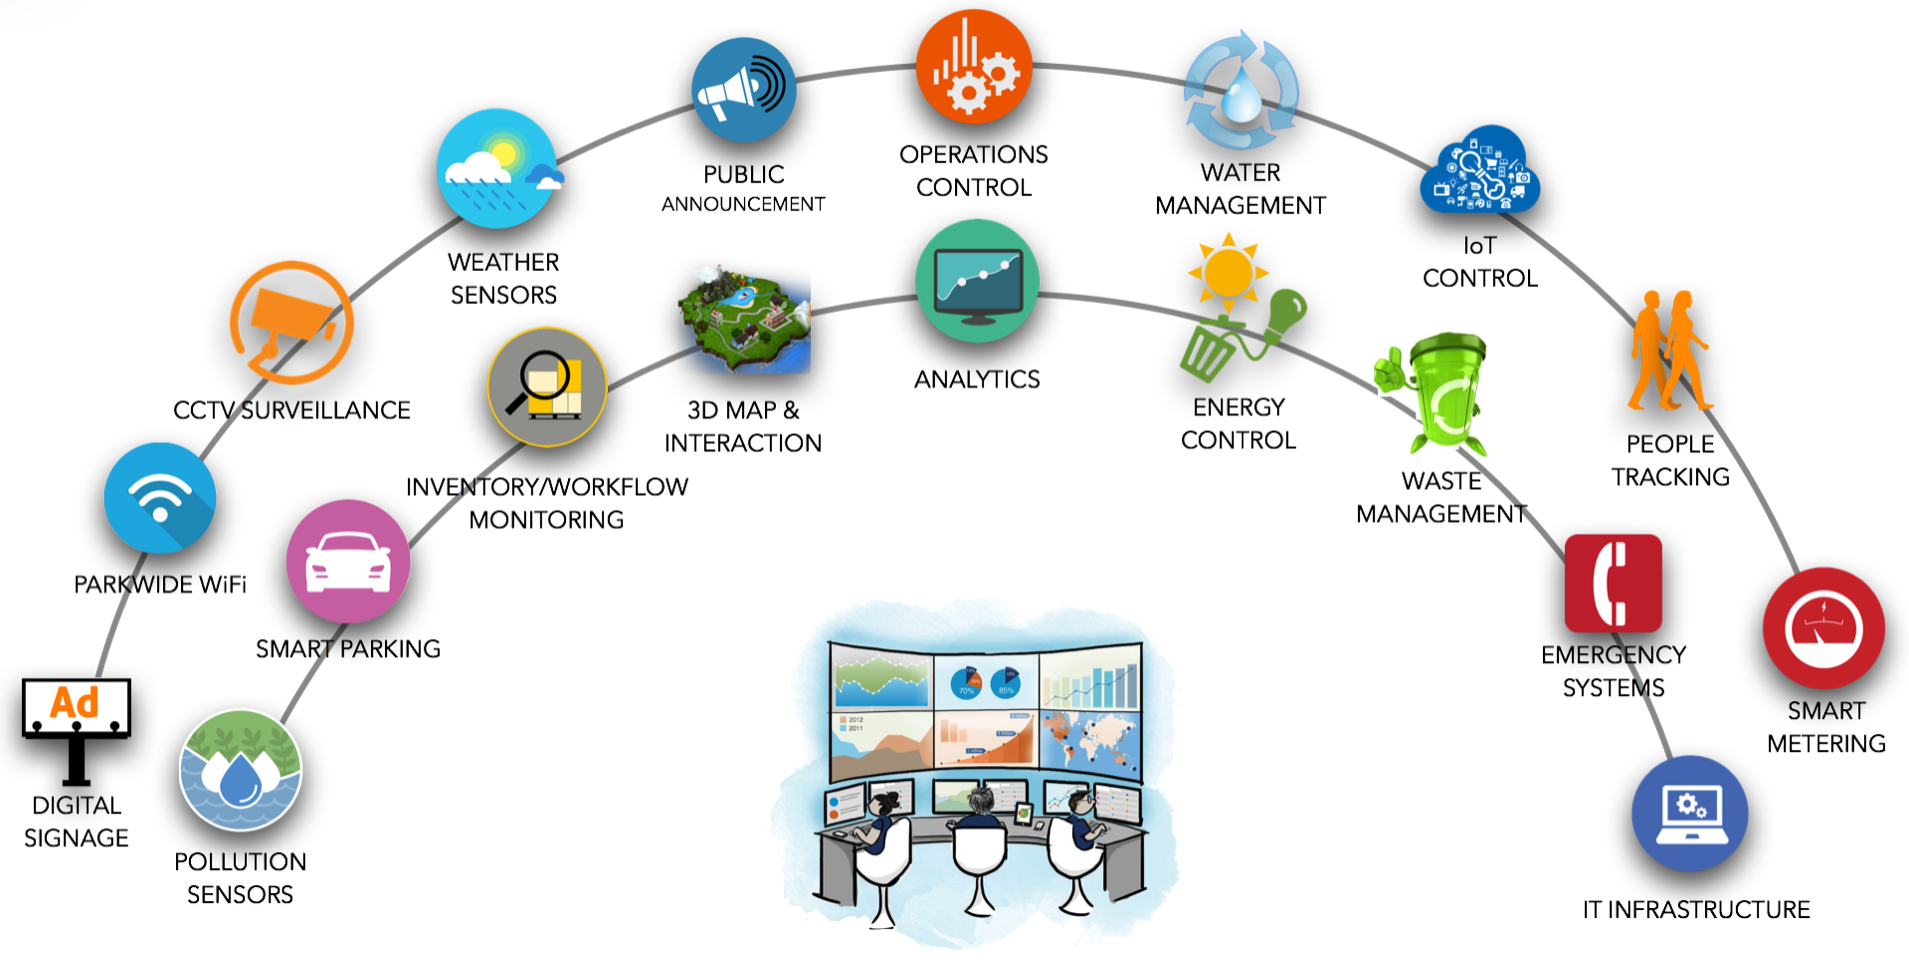
\includegraphics[width=0.9\columnwidth]{images/SmartCity.png}
\caption{Sources of data for smart city management \cite{figureSourcesofData}}
\end{figure}
The term "open data" is not confined to government data alone; it extends to the private sector, where recognition of the potential benefits of sharing data is growing. Both public and private entities now acknowledge the value of data as a key resource that enhances efficiency and effectiveness in various everyday activities. In the context of smart cities, the number and diversity of stakeholders involved are notably higher than in traditional private business cases. This includes utility companies, transport providers, mobile phone operators, social media platforms, financial institutions, surveillance and security providers, emergency services, and, notably, the citizens themselves. The collective appreciation of the value of data underscores its central role in shaping the present and future of smart urban environments.

\subsection{International Collaboration: Open Data and Sustainable Development Goals}
Open Data initiatives are also promoted by governative organizations, such as EU, giving the members a Directive (2019/1024)\cite{EU2019Directive}, based on the general principle that public data and data funded with public funds should be reusable for commercial or non-commercial purposes. The directive promotes the use of open data presented in open formats that can be freely used and shared for any purpose.

\begin{itemize}
    \item \textbf{Format and Accessibility}: Public entities and public enterprises must make documents available in any language or pre-existing format. Electronic availability through open, machine-readable, accessible, searchable, and reusable formats, along with metadata, is encouraged.
    \item \textbf{Practical Provisions for Reuse}: Public entities must examine reuse requests, making documents available electronically within a reasonable timeframe. Measures to facilitate online search and retrieval of documents are required.
    \item \textbf{Dynamic and Real-time Data}: Dynamic data must be immediately available through application programming interfaces (APIs) and, if necessary, as bulk downloads.
    \item \textbf{Research Data}: Member States must adopt national policies to open up publicly funded research data following the FAIR\footnote{FAIR data are data which meet principles of findability, accessibility, interoperability, and reusability (FAIR).} principles, considering intellectual property rights, personal data protection, privacy, security, and legitimate commercial interests.
    \item \textbf{Non-Discrimination and Transaction Equity}: Reuse of documents is open to all market actors without discrimination. Exclusive rights in contracts between public entities or public enterprises and third parties are generally discouraged, and specific transparency requirements apply to allowable agreements.

    \item \textbf{High-Value Data Sets}: Documents associated with significant socioeconomic benefits should be made available under particularly favorable reuse conditions. The directive mandates the European Commission to adopt a list of high-value data sets, covering six thematic categories (geospatial, earth and environment observation, weather, demographic, mobility, business and company ownership data).
\end{itemize}

Moreover, open data plays a crucial role in advancing the global pursuit of sustainable development, aligning closely with the United Nations Sustainable Development Goals (SDGs)\cite{sdgs}. By fostering transparency, \textbf{collaboration}, and innovation, open data emerges as a powerful catalyst for addressing the complex challenges outlined by the SDGs. It transcends borders, providing a shared resource that empowers individuals, communities, and nations to collectively work towards a more sustainable and equitable future. The inherent openness of data facilitates a deeper understanding of societal issues, allowing stakeholders to make informed decisions and implement effective solutions. This transparency promotes accountability among governments, encourages citizen engagement, and contributes to the common goal of creating inclusive and fair societies. Moreover, the accessibility of data enables the identification of gaps and disparities, facilitating targeted interventions to uplift marginalized communities and bridge socioeconomic divides. Furthermore, open data fosters collaboration on a global scale. By breaking down barriers and facilitating the exchange of information, it enables nations to learn from each other's successes and challenges. This collaborative approach is essential for tackling transboundary issues such as climate change, poverty, and health crises, which are central to the SDGs. Open data can become a unifying force that empowers nations to collectively address shared challenges and work towards common objectives.

\subsection{Application examples of Open Data}

In the realm of real-world application of open data, a myriad of applications have emerged, showcasing the transformative power of data-driven solutions across diverse domains. Let's explore seven examples of applications that highlight the versatility of open data in addressing real-world challenges.
In the realm of real-world application of open data, a myriad of applications have emerged, showcasing the transformative power of data-driven solutions across diverse domains. Let's explore seven examples of applications that highlight the versatility of open data in addressing real-world challenges \cite{electronics10232997}.
\begin{enumerate}
\item \textbf{Air Quality Monitoring Systems:}
   Numerous cities have embraced open data to develop low-cost air pollution monitoring systems. By integrating data from various sources, such as sensors scattered around the city, these systems enable real-time tracking of air quality indices in each area, helping authorities and citizens make informed decisions about outdoor activities and health precautions.

\item \textbf{Traffic Flow Optimization:}
   Leveraging open data on traffic patterns and atmospheric conditions, smart city initiatives aim to optimize traffic flow. By employing machine learning algorithms, these projects forecast congestion-prone areas, facilitating dynamic traffic signal control, as we have seen in the Singapore example. The goal is not only to reduce travel time but also to minimize vehicular emissions and alleviate pollution.

\item \textbf{Urban Green Spaces Mapping:}
   Open data plays a crucial role in mapping and monitoring urban green spaces. By utilizing satellite imagery and geospatial data, projects identify areas with vegetation cover, helping city planners enhance green infrastructure. This, in turn, contributes to improved air quality and overall environmental well-being.

\item \textbf{Water Resource Management:}
   Machine learning algorithms applied to open data sets can extract valuable insights for water resource management. By analyzing satellite images and GIS data, projects identify non-water bodies like urban areas and vegetation. This aids in efficient water resource management, preventing contamination and ensuring sustainable use.

\item \textbf{Accident Prediction Models:}
   Open datasets of large cities are harnessed to create high-resolution accident prediction models. Machine learning methods are employed to predict accident-prone zones, contributing to proactive measures for improving road safety.
   
\item \textbf{Flood Monitoring and Prediction:}
   Open data, including weather information and satellite imagery, is utilized to develop flood monitoring and prediction systems. Machine learning models can effectively classify images related to drain blockages and abnormal water levels, assisting in early detection and response to potential flooding events.

\item \textbf{Urban Energy Consumption Modeling:}
   Utilizing open data, particularly smart metering information and building footprints, projects develop models for predicting urban energy consumption. Machine learning algorithms enable accurate forecasting of energy demand, aiding in the implementation of energy-efficient practices and reducing the environmental footprint of urban areas.
\end{enumerate}

These real-world projects demonstrate the impactful synergy between open data and innovative technologies, addressing several challenges related to urbanization and pollution.

\section{Pollution monitoring in smart cities}

As mentioned above, one of the critical challenges lies in effectively build an air quality management system. This system plays a pivotal role in detecting hazardous gases, enabling residents to make informed decisions about their living spaces. Additionally, it serves as a catalyst for governmental interventions aimed at reducing the sources of these harmful emissions.

The traditional notion of literature often depicted industrial zones as having precarious air quality, while green areas were considered healthier. However, in contemporary times, this paradigm has shifted, and even green spaces are not exempt from air quality concerns \cite{rhaiemair}. Clean and fresh air is a fundamental element for a healthy life, but numerous factors impact its purity.

Air pollution emerges as a critical health issue in cities, causing significant premature deaths globally. The World Health Organization (WHO) reports that outdoor Ambient (outdoor) air pollution is estimated to have caused 4.2 million premature deaths worldwide in 2019\cite{WHO2018AirPollution}. Urban areas grapple with air pollution, with a particular focus on Particulate Matter (PM), especially PM 2.5 and PM 10, which can penetrate the respiratory system.

To address these challenges, smart cities must prioritize the monitoring of environmental conditions. Deploying a network of low-cost air quality monitoring sensor nodes becomes essential to identify pollution sources and mitigate their impact. By detecting sources of pollution, cities can take corrective actions, enhancing environmental health. Implementing disaster detection systems, such as flood and precipitation monitoring solutions, provides citizens with advanced warnings. This holistic approach allows authorities to make informed, data-driven decisions for infrastructure planning and policy formulation. Continuous study of air quality variables is crucial to effectively classify cities based on the safety and well-being of their residents.

\subsection{Main pollutants in urban spaces}

In air quality studies, some pollutants emerge as more impactful on public health, making them a threat to keep an eye on. Here are six of them:
\begin{itemize}
    \item \textbf{Ozone (O\textsubscript{3})}: this gas poses, especially on hot days, health risks by causing respiratory issues such as coughing, difficulty breathing, and lung inflammation.
    \item \textbf{Nitrogen dioxide (NO\textsubscript{2})}: mainly emitted from fuel combustion, irritates human airways and can worsen respiratory conditions, especially asthma, causing short-term exacerbations and respiratory symptoms.
    \item \textbf{Solfure dioxide (SO\textsubscript{2})}: subproduct of fuel combustion in various sources, irritates eyes and the respiratory system. Low concentrations affect the eyes and upper respiratory tract, while higher levels can lead to nasal irritation, bronchitis, and lung disease.
    \item \textbf{Carbon monoxide (CO)}: this pollutant derives from fossil fuels, common in traffic, harms cardiovascular health, causing issues for individuals with heart disease and affecting anyone with vision and cognitive problems at high levels, potentially leading to fatalities.
    \item \textbf{Fine particulate matter (PM\textsubscript{2.5})}: tiny airborne particles from various sources, can enter the respiratory system and bloodstream, leading to health issues such as respiratory and cardiovascular problems.
    \item \textbf{Particulate matter (PM\textsubscript{10})}: larger than PM\textsubscript{2.5} particles, includes various sources like combustion and industrial processes. While primarily affecting the upper respiratory tract, PM\textsubscript{10} poses health risks, especially for those with respiratory conditions. 
\end{itemize}


In brief, the discussed urban pollutants can significantly impact public health and well-being. The widely used measure to assess overall air quality, is the Air Quality Index (AQI), which provides a comprehensive score that helps the public grasp the current state of the air they breathe.

\subsection{The Air Quality Index}

The computation of the Air Quality Index (AQI) relies on the measurement of air pollutant concentrations over specific time intervals, obtained from air monitors or models. The combination of concentration and time represents the dose of the air pollutant. The health effects associated with pollutants are determined through epidemiological research. It is important to note that different pollutants have varying impacts, and the conversion function from concentration to AQI is different for each pollutant. AQI values are categorized into ranges, each associated with a descriptor, color code, and standardized public health advisory.
On days when the AQI is predicted to be elevated due to fine particle pollution, agencies or public health organizations may take several measures:
\begin{compactenum}
    \item Advise sensitive groups, such as the elderly, children, and individuals with respiratory or cardiovascular issues, to avoid outdoor exertion.
    \item Declare an "action day" to encourage voluntary measures, such as using public transportation, to reduce air emissions.
    \item Recommend the use of masks outdoors and air purifiers indoors to prevent fine particles from entering the lungs.
\end{compactenum}
In cases of very poor air quality, such as during air pollution episodes, when the AQI indicates a potential for significant harm to public health from acute exposure, agencies may implement emergency plans. These plans can include orders for major emitters, like coal-burning industries, to curtail emissions until hazardous conditions improve.
It's important to note that not all air contaminants have an associated AQI. Many countries monitor pollutants such as ground-level ozone, particulates, sulfur dioxide, carbon monoxide, and nitrogen dioxide, calculating air quality indices for these substances.
There is also a website \cite{Airqualityindexwebsite} that allows government agencies worldwide to submit real-time air monitoring data. This platform employs a common definition of the air quality index, facilitating a standardized display of information.

Each country sets its air quality index thresholds based on factors such as territorial morphology. In the European Union (EU), specific values have been established, ranging from 1 (good) to 6 (extremely poor), as depicted in the table \ref{fig:euaqitable}. The index for each pollutant is determined independently based on concentrations, with higher concentrations corresponding to higher index values. The European Air Quality index for a specific hour is simply the highest value among the five individual pollutant indexes calculated during that hour. Similarly, the daily European Air Quality index is the highest value of the overall hourly index for the corresponding day.
\begin{figure}
    \centering
    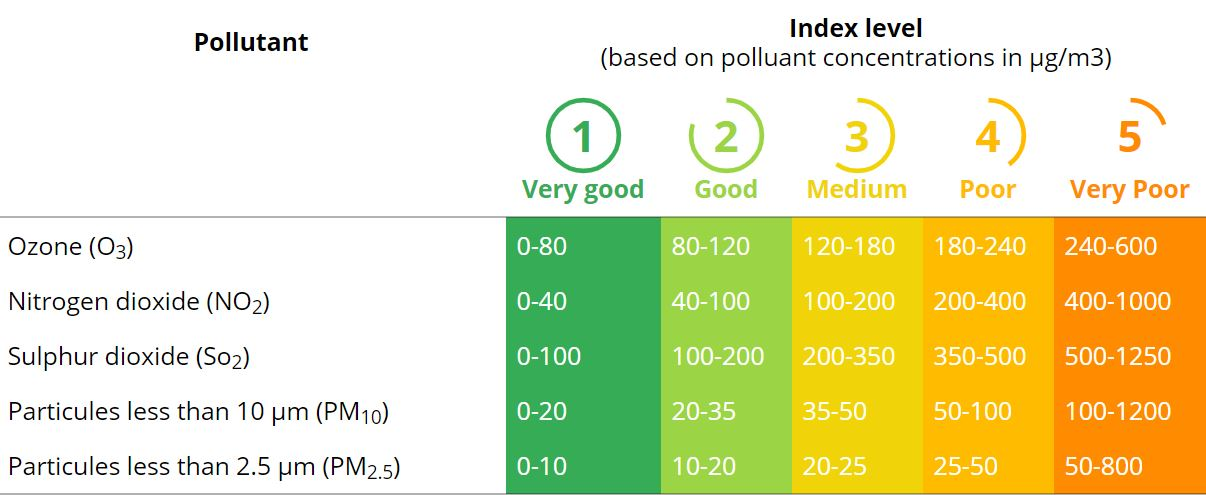
\includegraphics[width=1\linewidth]{images/airqualityindexcalc.png}
    \caption{European air quality index thresholds}
    \label{fig:euaqitable}
\end{figure}

As we can see, Europe does not take into account the measurements of CO concentration for the calculation of the Index.

\subsection{Beijing example}

In 1998, Beijing initiated a concerted effort to address air pollution, acknowledging the environmental issues confronting one of the world's largest and fastest-growing cities. Initially grappling with pollution driven by coal combustion and vehicular emissions, surpassing national limits, the city undertook a series of measures over the subsequent 15 years. These efforts aimed at optimizing energy infrastructure, controlling coal-fired pollution, and regulating vehicle emissions. By 2013, significant reductions in air pollutants were evident, meeting national standards for specific pollutants \cite{CCAC2019}.
However, the pivotal moment materialized in 2013, marked by Beijing adopting more systematic and intensive measures for air pollution control. By the close of 2017, there was a notable 35\% decrease in fine particulate pollution (PM\textsubscript{2.5}). This achievement resulted from targeted actions like controlling coal-fired boilers, advocating for cleaner domestic fuels, and restructuring industries. During this timeframe, emissions of sulfur dioxide (SO\textsubscript{2}), nitrogen oxides (NO\textsubscript{x}), particulate matter (PM\textsubscript{10}), and volatile organic compounds in Beijing saw a substantial decrease. Beijing's approach to air quality management distinguishes itself with robust monitoring, pollution source identification, emission inventories, comprehensive legal standards, and stringent environmental law enforcement. 

\begin{figure}
    \centering
    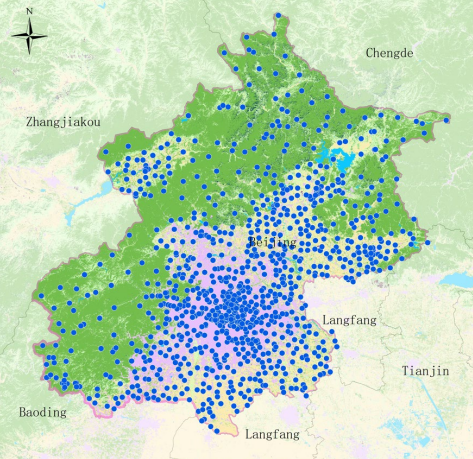
\includegraphics[width=0.5\linewidth]{images/beijingsensors.png}
    \caption{Beijing's high-density sensor-based PM\textsubscript{2.5} monitoring network \cite{UNEnvironment2019}}
    \label{fig:beijingsensors}
\end{figure}

Despite recognizing achievements, the Beijing municipality acknowledges persistent challenges, particularly concerning PM\textsubscript{2.5} concentrations that still fall short of national standards, and because episodes of heavy pollution persist during autumn and winter. Nevertheless, Beijing affirms its commitment to sharing accumulated knowledge and experiences on air pollution with other developing cities, emphasizing that addressing air quality issues is an ongoing and long-term process.

\section{Previous works on air pollutants forecasting}
\label{cap1:sota}
Over the years, numerous authors have endeavored to address the challenge of predicting pollutants in cities using various methods, encompassing both classical and deep learning techniques. The primary obstacles encountered in this task include:

\begin{enumerate}
  \item \textbf{Missing Data}, arising from erroneous observations or sensor unavailability.
  \item \textbf{Collinearity} between the target variables.
  \item \textbf{Complex and Multiple Seasonality Patterns}, which adds another layer of complexity.
\end{enumerate}

The models employed must demonstrate proficiency in learning from extended sequences to make accurate forecasts. Additionally, they should incorporate mechanisms that facilitate the interaction among features for enhanced predictive capabilities.

\textbf{Classical models}, like ARIMA (referenced in \cite{DIAZROBLES20088331} and \cite{Jodar2013}), have demonstrated the ability to predict the overall trend of time series data. However, they often fall short in predicting peaks, possibly due to their inability to capture the nonlinear patterns typically present in air quality time series. Moreover, the datasets used in these analyses focused on univariate regression problems, predicting each pollutant individually. To address these limitations, the papers suggest an innovative approach: combining an artificial neural network architecture with the ARIMA model. Additionally, meteorological variables are incorporated as external regressors to enhance predictive accuracy.\\

With increased computing capacity and rapid growth in deep learning studies, the development of \textbf{more sophisticated network architectures} has become possible. These architectures can capture complex patterns and combine spatial and temporal features of this kind of data.
Many approaches include the use of \textbf{Long-Short Term Memory (LSTM) networks}, combined with various mathematical and statistical techniques.

\noindent K\"{o}k et al. \cite{8258144} use a simple LSTM to make one-step-ahead predictions of Ozone and NO\textsubscript{2}. Then the predictions are used to classify the AQI for the predicted day.

\noindent Han et al. \cite{9127775} proposed a combination of Bayesian, domain-specific knowledge, and deep learning to reduce error. The approach enables the fusion of different forecast strategies thanks to probabilistic Bayesian modeling, reducing overfitting and providing a measure of uncertainty.

\noindent Song et al. \cite{lstmkalman} introduced a time prediction model, LSTM-Kalman, for forecasting time series data with long-term and short-term characteristics. Leveraging LSTM's memory feature, the model captures and stores information from previous data, utilizing it in subsequent processing to obtain the underlying time series. Kalman filtering is used to dynamically adjusts the LSTM-processed data sequence, yielding an improved predicted value.

\noindent Yin et al. \cite{Yin2020} presented DAEDN (Denoising Auto Encoder Deep Network), a novel air pollutant prediction model based on bidirectional LSTM networks. Trained on 5 years of Beijing's PM\textsubscript{2.5} data, DAEDN outperforms unidirectional LSTM with a 7.33\% reduction in RMSE and a 5.87\% reduction in MAE. The model effectively extracts stable features from noisy input, considering time series properties and integrating environmental big data sources such as weather data.

\noindent Jin et al. \cite{WaveletNLSTM} suggested a neural network architecture for multivariate, multi-step predictions using Wavelet transform to decompose the time series of pollutants. They then input the components into a Nested-LSTM layer, allowing an extension of the memory capability of the traditional LSTM, and combine the features obtained from each layer in a shared layer before the output layer.

\noindent Similarly, Zeng et al. \cite{ZENG2022108822} proposed a model that integrates the extended stationary wavelet transform (ESWT) and the nested long short-term memory (NLSTM) neural network for PM\textsubscript{2.5} forecasting. The authors claim that the method outperforms state-of-the-art forecasting methods in terms of different error metrics, such as absolute error, R2, MAE, RMSE, and MAPE.\\


In the last four years, as the availability of data increased, new approaches taking into account the \textbf{spatial information} of the data, obtained by multiple stations observing at the same time, occurred:

\noindent Qi et al. \cite{graphlstm1}, proposed a hybrid model for spatiotemporal forecasting of PM\textsubscript{2.5} based on graph convolutional neural network and LSTM, which applies a Graph Convolutional Network (GCN) to extract the spatial dependence between different stations and LSTM to capture the time dependence between observations at different times. 

\noindent Wen et al. \cite{WEN20191091} suggested a Convolutional Long Short-Term Memory Neural Network Extended (C-LSTME), designed for predicting air quality concentration. To effectively capture both spatial and temporal aspects of the data, the model incorporates historical air pollutant concentrations from the current station, as well as those from adaptively selected k-nearest neighboring stations. The integration of Convolutional Neural Network (CNN) and LSTMs facilitates the extraction of high-level spatiotemporal features. Additionally, the model incorporates meteorological and aerosol data after the feature extraction before a multilayer perceptron (MLP) block, to enhance its predictive performance.

\noindent Wang and Han \cite{Wang2023} proposed a Dirichlet Graph Convolution Coupled Neural Differential Equation for Spatio-temporal Time Series Prediction. This GCCNDE model predicts by learning initial spatio-temporal features, mapping them to a high-dimensional space, modeling dynamic evolution with GAT and NDE, and obtaining final predictions by mapping the high-dimensional state back to the original space. It assumes shared spatial representations between adjacent time steps for effective prediction.

In this work, various model architectures for a multivariate multi-step forecasting has been tested, using both external features and historical values. In the next chapter a deep analysis of three air quality datasets will be conducted.
\newpage


















